\documentclass{article}
\usepackage{graphicx}
\usepackage{amsmath}

\begin{document}

\title{Trayectoria de una Bola de Billar}
\author{David Rivera Morales}
\date{\today}

\maketitle

\section{Problema}
Una bola de billar, en una mesa de billar, sigue el camino definido por \(c(t) = (|t|, |t−1/2|)\), donde −1 ≤ t ≤ 1. 

\section{Solución}
La trayectoria seguida por la bola de billar se puede visualizar en el siguiente gráfico:

\begin{figure}[h]
\centering
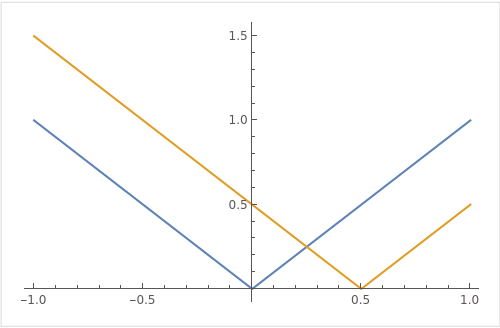
\includegraphics[width=0.5\textwidth]{image.png}
\caption{Trayectoria de la bola de billar. El eje horizontal representa el tiempo \( t \), y los dos ejes verticales representan las dos componentes de la trayectoria \( c(t) = (|t|, |t−1/2|) \).}
\end{figure}

\end{document}
